\begin{frame}{Conclusion}

	\begin{columns}
	
		\begin{column}{0.5\textwidth}
		
			\newcolumntype{a}{>{\columncolor[gray]{0.8}}c}	
			\begin{table}
				\begin{tabular}{c|c|a|c|c|c}	
													&				 	& Sensitivity 	&  1				&				&  n 		\\\hline
					\cellcolor[gray]{0.8}Privacy 	& Attitude			& User / Item 	& msg1			& ... 			& msgn  		\\\hline
					P1								&  1	 				& User 1			& 				&				&			\\\hline
					...								& 					& 				& 				&	R(i,j)		&			\\\hline
					PN								&  N	 				& User N			& 				&				&	
		
				\end{tabular}
				\caption{\label{tab:widgets} An example table.}
			\end{table}		
		
			\begin{figure}
				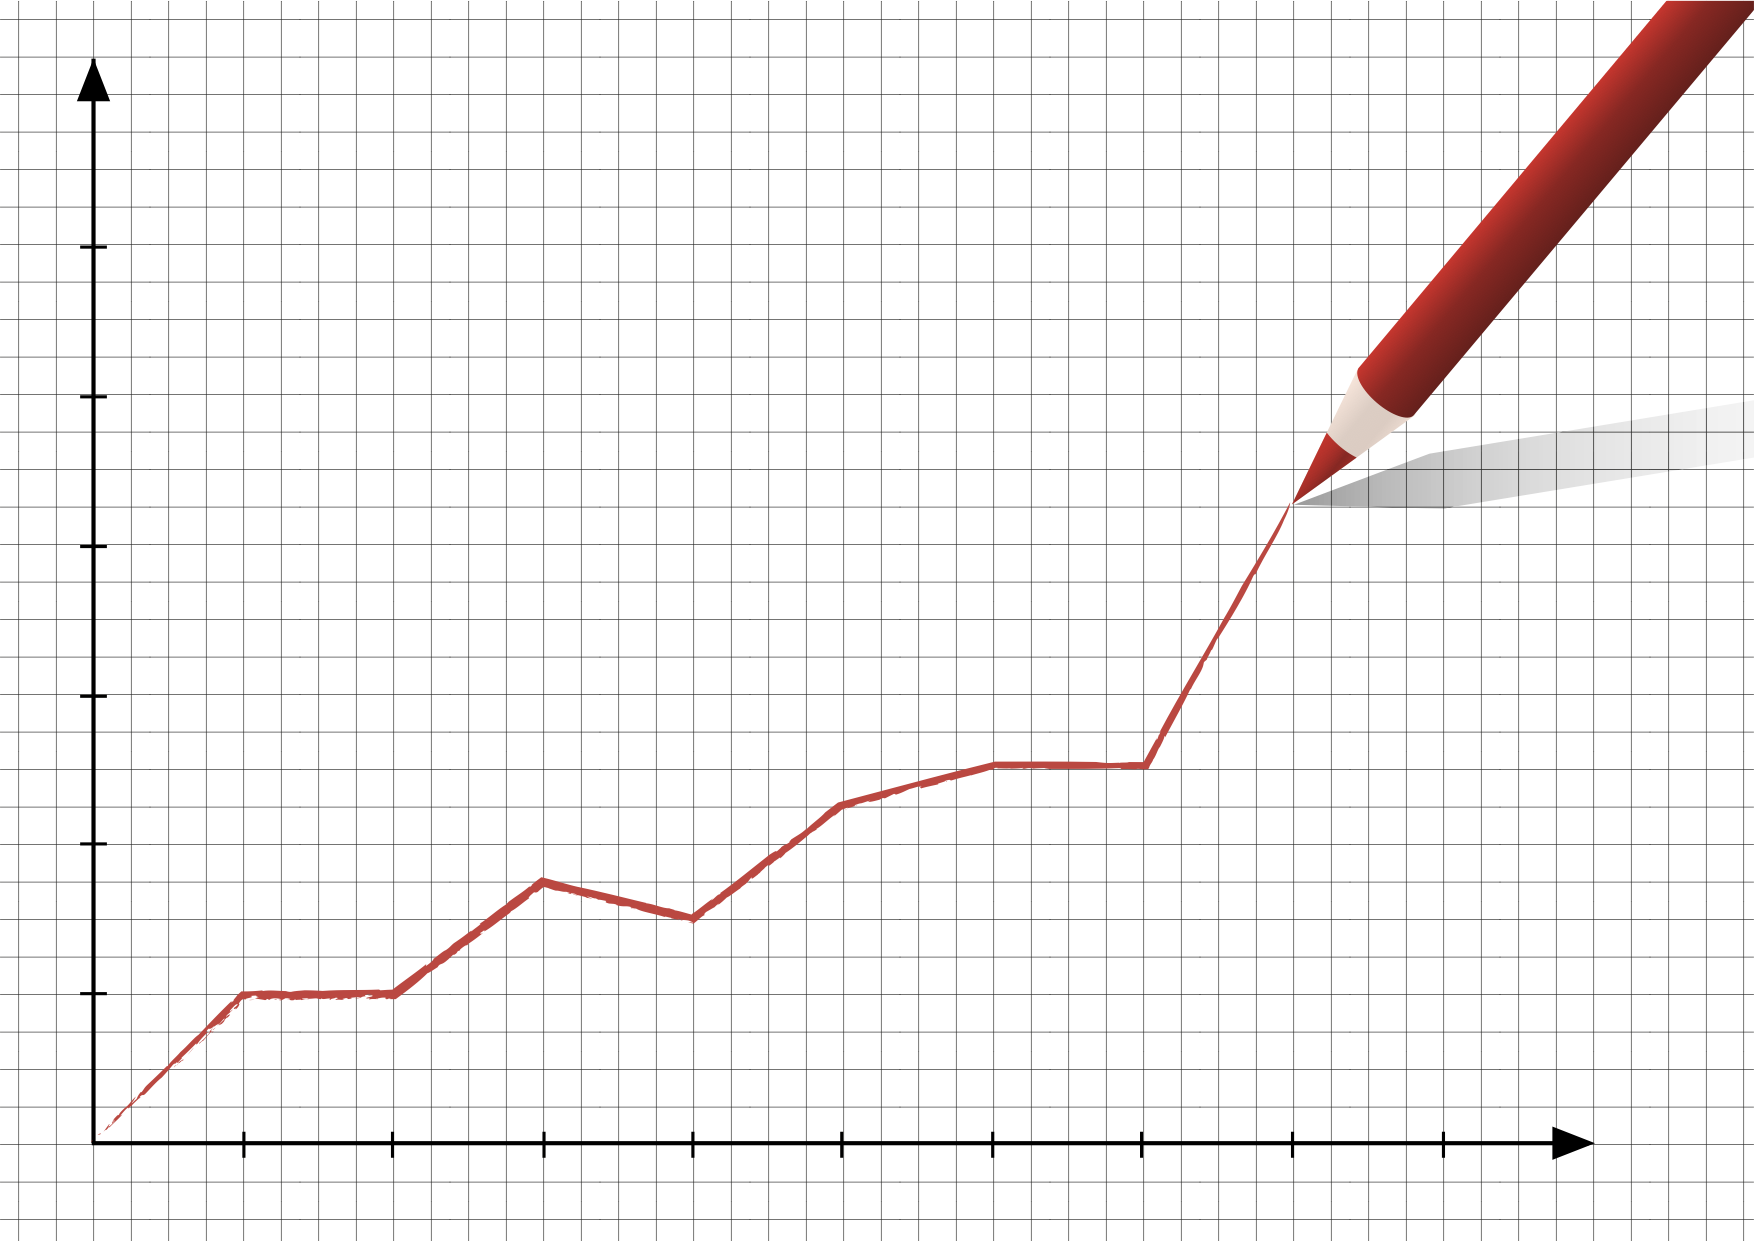
\includegraphics[scale=0.09]{res/mail.png}
				\caption{\label{fig:g}Cag.}
			\end{figure}
			
		\end{column}
		
		\begin{column}{0.5\textwidth}

			\begin{figure}
				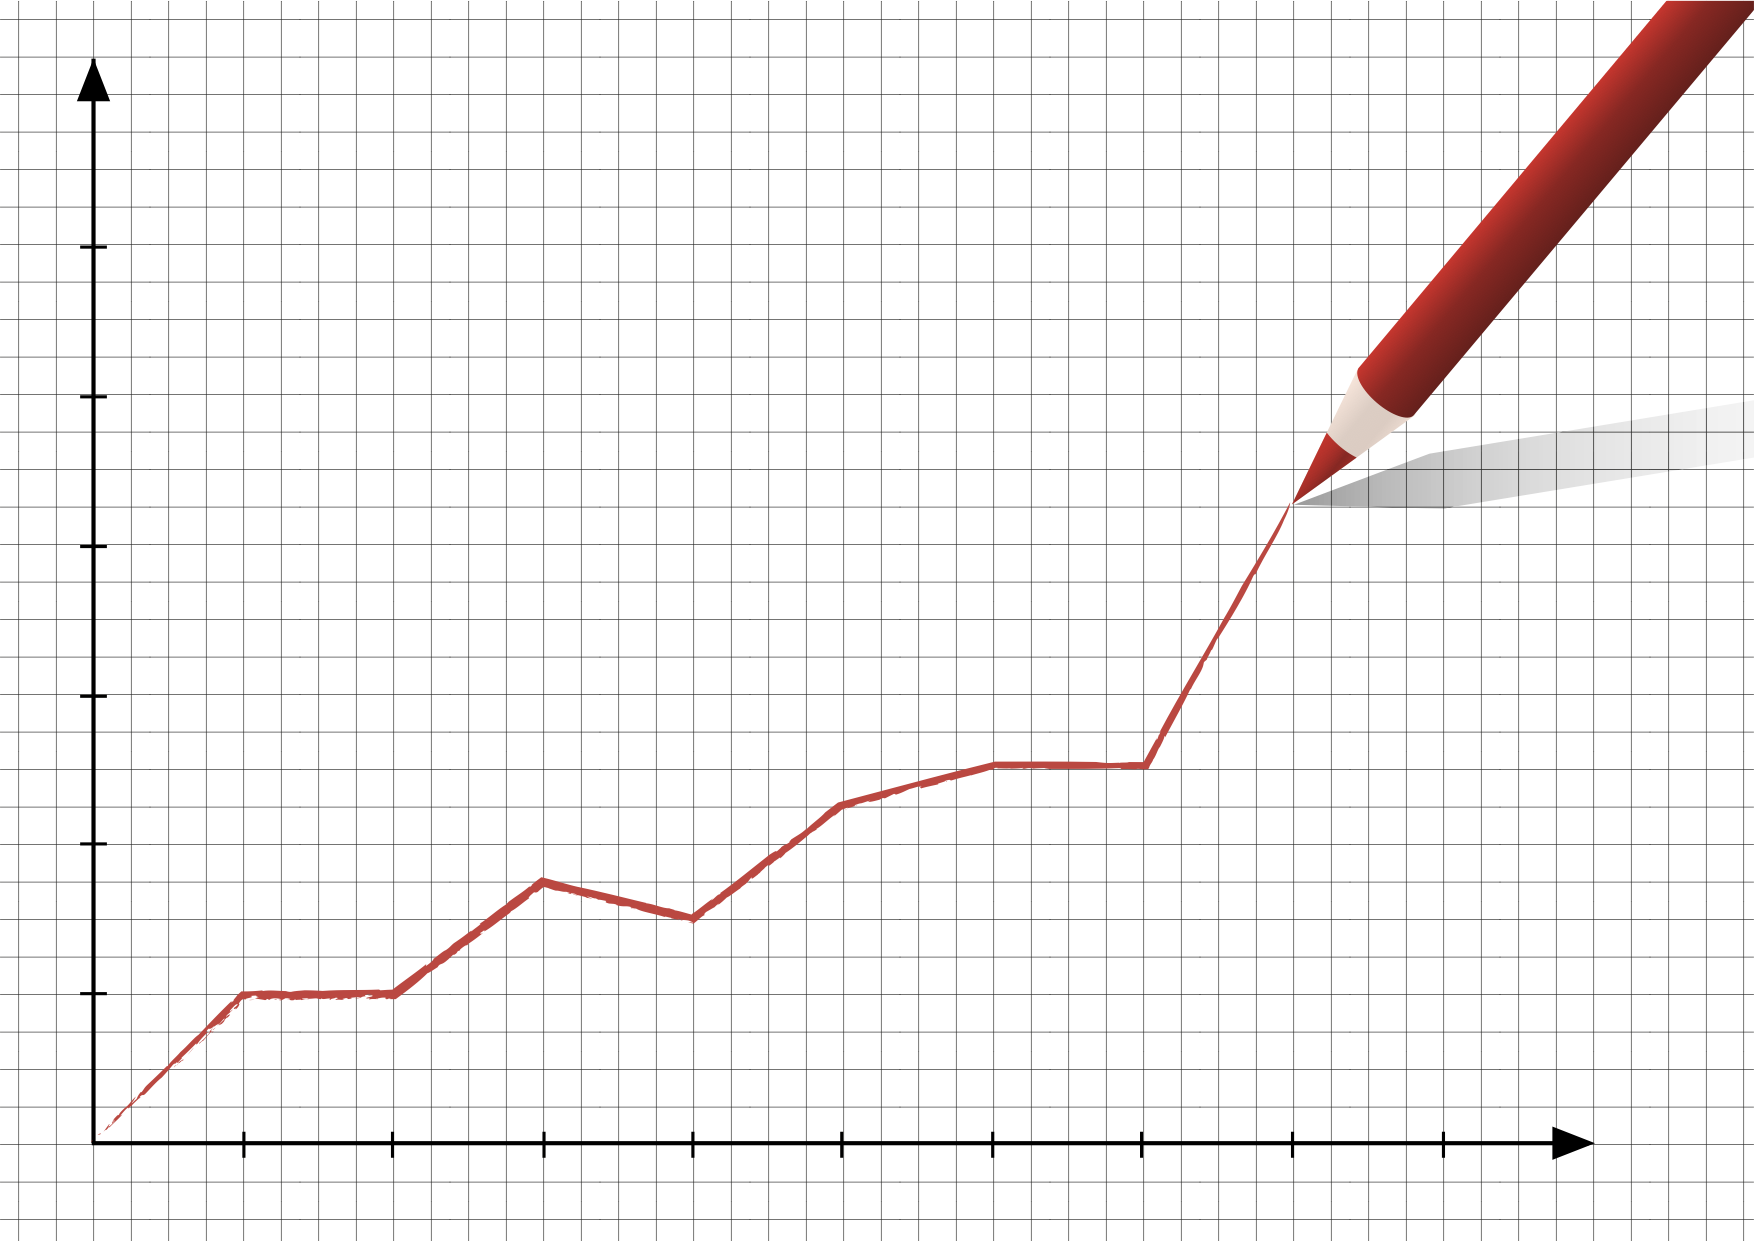
\includegraphics[scale=0.09]{res/mail.png}
				\caption{\label{fig:g}Cag.}
			\end{figure}
			
			\begin{figure}
				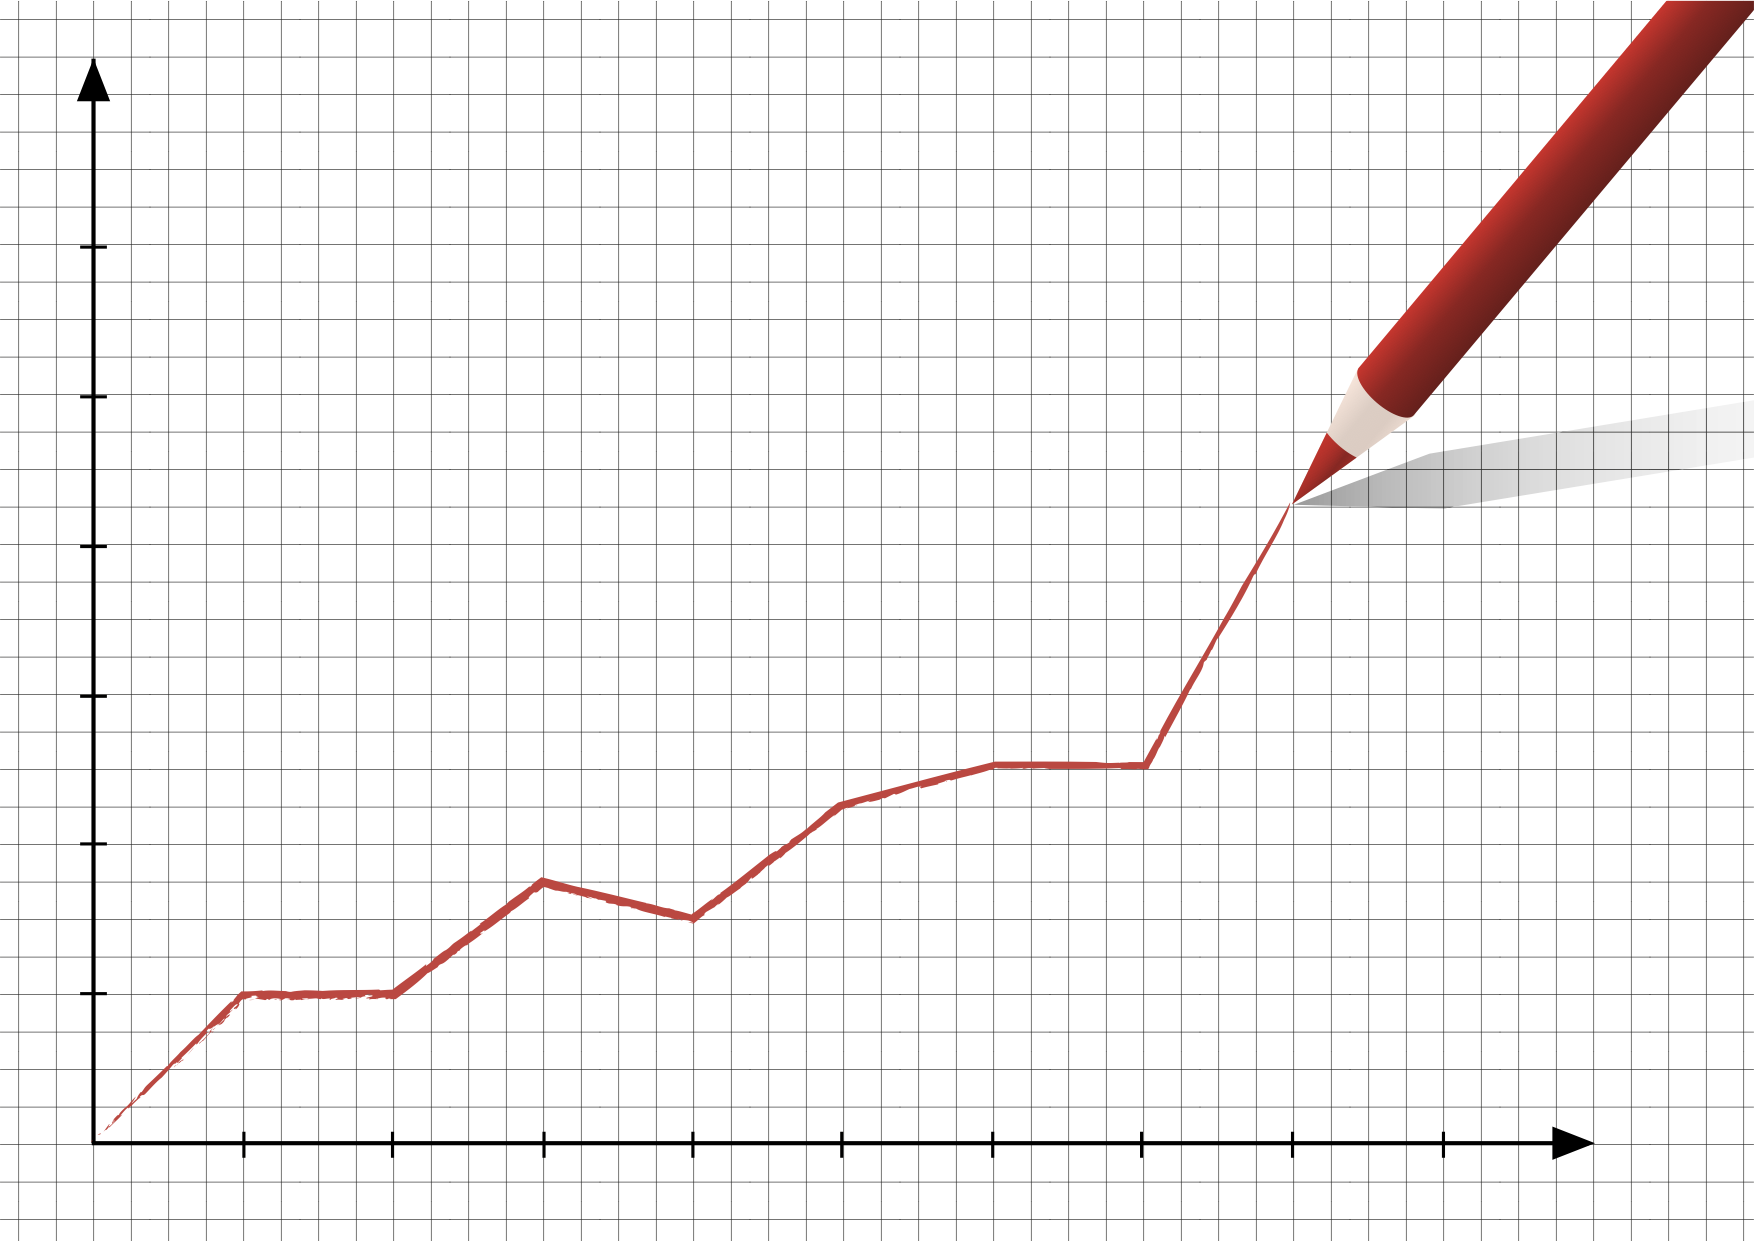
\includegraphics[scale=0.09]{res/mail.png}
				\caption{\label{fig:g}Cag.}
			\end{figure}

		\end{column}
	\end{columns}

	% Commands to include a figure:
	%\begin{figure}
	%\includegraphics[width=\textwidth]{your-figure's-file-name}
	%\caption{\label{fig:your-figure}Caption goes here.}
	%\end{figure}
	


\end{frame}

